\documentclass{sig-alternate}
\usepackage{graphicx}
\usepackage{listings}
\usepackage{syntax}
\usepackage{listing}
\usepackage{url}
\usepackage{framed}
\usepackage{verbatim}
\usepackage{hhline}
\usepackage[]{algorithm2e}
\usepackage{makecell}
\usepackage[capposition=top]{floatrow}

\begin{document}

\title{Joint Optimization of Link and Node resource in a Network}

\begin{comment}
\numberofauthors{1} 
\author{
\alignauthor X. Kelvin Zou, Yonatan Naamad, Moses Charikar, Jennifer Rexford\\
\affaddr{Princeton University}\\
\email{\{xuanz, ynaamad, moses, jrex\}@cs.princeton.edu}
}
\end{comment}
\maketitle
\begin{abstract}

\end{abstract}

\section{Introduction}

Network has been long treated as a graph problem, max flow and shortest path originated from theory research have been widely used in network design and operation. Nevertheless, the simple graph model does not capture the whole story, network flow is more than simply a flow; in-network process for flows have played a crucial role in today's network. Network appliances(e.g. firewall, proxy, intrusion detection and prevention system) are named "middleboxes" after their position: in the middle of the network. Middleboxes are pivotal components for in-network process and therefore essential to today's network.

Some studies show that the market for middleboxes will grow up to ten billion dollars\cite{SecurityMarketResearch,COMB2012}. There is a strong reason to argue that middleboxes are no longer "second class citizen" in networking design and deployment, and we should treat them with equal importance when designing a network. In particular, how to route and process the flows should be jointly optimized during networking design.

Traditionally, those middleboxes had to use specialized hardware to get ideal performance, for instance, transcoding requires high computational power and deep packet inspection consumes a lot of memory. Due to the high cost of the specialized hardware, network designs are restricted by the limited number of middleboxes and their functionalities. Network operators tend to place middlebox with great caution and calculation, and in many cases middleboxes are simply placed at chokepoints such as gateway, so flows can share the use of same middleboxes. Choke point placement achieves efficient usage and coverage of middleboxes, the tradeoff is its vulnerability to single point failure. Some new approaches use the idea of Software-Defined Network (SDN), and take advantage of its centralized view of network and provide more freedom for middlebox placement while forcing the traffic to steer to middleboxes, however this approach inevitably creates excessive bouncing traffic\cite{SIMPLE2013,FLOWTAGS2014}.

Network function virtualization has taken place, people proposed various designs of virtualization, e.g. OpenVSwitch\cite{openvswitch}, modular middlebox\cite{COMB2012, clickos} . Middleboxes are suitable for virtualization in nature: unlike switch or router which only requires simple forwarding actions, middleboxes require more advanced functions and not simply just I/O bounded, CPU and memory in many cases are the bottleneck. As the hardware capability grows and the gap between hardware and software solutions closes, it is not hard to imagine a wider deployment of virtual middleboxes. 

Though the virtualization is trending, people still build the network around router and switch with the old mindset of using physical middlebox, and the placement has not changed much. Outsourcing to cloud or handling at end machines in a elastic manner has been proposed but it imposes high latency and redundant traffic\cite{APLOMB2012, ANANTA2013}. As virtualization enables elasticity and divisibility, it makes middlebox placement more flexible, we argue that all middlebox instances can be run anywhere in the network, by doing that, we can:
\begin{itemize}
  \item \textbf{Eliminate single point failure of middlebox}
  
  Traditional network meticulously places middlebox at choke point shared by many flow and thus force the traffic to go through. This system eliminates the existence of choke point and is easier to implement a fault tolerant system.
  
    \item \textbf{Reduce unnecessary bouncing traffic} 
  
  Some networks steer traffic to some middlebox and may add redundant load on the network and extra latency for each flow. We can take advantage of virtualization and placement freedom to reduce unnecessary traffic bouncing. 
  
  \item \textbf{Ease middlebox policy enforcement and load balancing}

Current middlebox policy enforcement is implemented by forcing traffic go through each middlebox, e.g. firewall following proxy is done by force traffic go through firewall first and then proxy. In this system we can simply run different VM instances at the same node and enforce the policy. Dynamic spinning or closing a middlebox VM at nodes also makes load balancing easier.
\end{itemize}



\section{Network Model and Assumptions}
\subsection{Network Assumptions}
If we review the network model without middleboxes, it is essentially composed of nodes and links, and feasible flow problem is asking whether a flow pattern is feasible given constraints of link bandwidth. Max flow model\cite{FordFulkerson, Edmonds1972} has been widely applied in network traffic engineering. Although this model is well studied, it does not capture the whole story of network traffics: many network flows need to be processed in someway by some middleboxes along the path. 

Here we need to revise the network model. Since here the emphasis is to derive the best model for adding middlebox into abstraction, we make some basic assumptions for simplicity. All the flows are infinitely divisible and they can be split at any place in any fractional manner. The in-network processing demand for middlebox is proportional to the flow size, which means a flow of two units require twice as much processing capacity as flow of one unit. This assumption holds for most cases where middleboxes processing is per-packet based. We also assume that middlebox processing capacity and demand is homogenous, a reasonable assumption in the context of virtualization. Note that here different middleboxes might be constrained by different resources and we can solve this problem by finding the best way of calculating capacity via dominant resource or other resource allocation approach. We denote $r_i$ as flow rate for flow i, and $d_i$ as in-network processing demand for middleboxes, and we can also derive $q_i = \frac{d_i}{r_i}$ based on the assumption. 

\begin{figure}
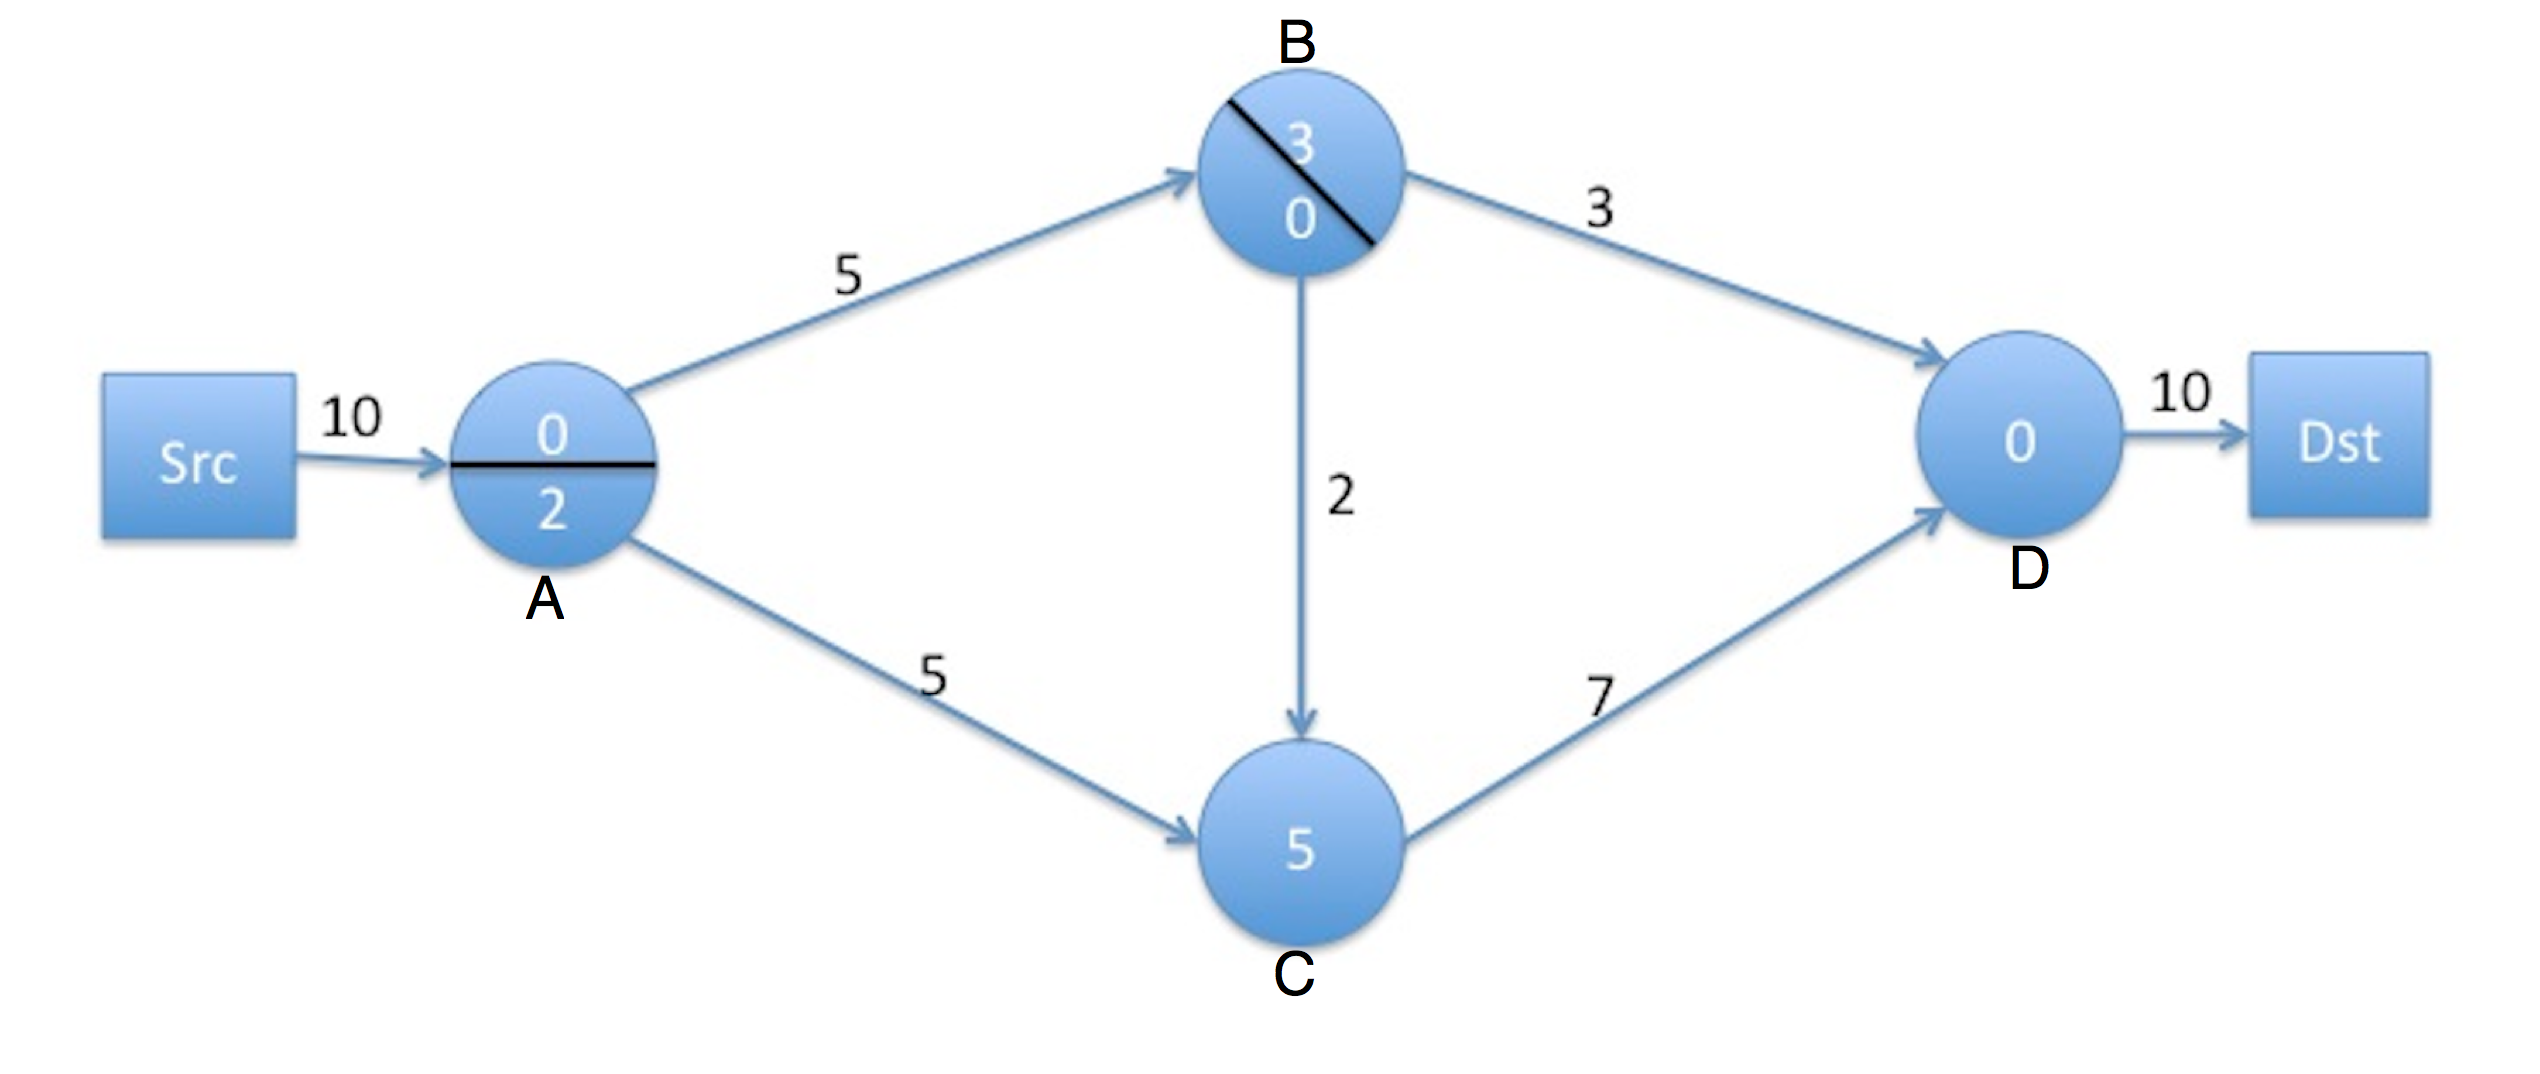
\includegraphics[scale=0.19]{demo.png} 
\caption{Simple example for graph model \label{figure}}
\floatfoot{If C(A)=2, C(B) =3, C(C)=5, all B(e) =10, one optimal solution would be 10 units of flow from src->A, at A 2 units processed and 3 units unprocessed flows send to C and 5 units unprocessed to B, at B 3 units processed sent to D and 2 units unprocessed to C, at C all units are processed along with 2 already processed flow (from A) sent to D.}
 \end{figure}
 

\subsection{Graph Model}


To integrate the middlebox into the graph model, we need to convert middleboxes to nodes or links. The role middlebox plays mathematically in a graph is quite different from links. Unlike simple flows where it is strictly constrained by the bottleneck link bandwidth, flow in-network processing is handled in a cumulative manner, in other words, it is constrained by the sum of all processing capacity of middleboxes on a path. From this point of view middleboxes can be treated as nodes and we can set different constraints for nodes in the graph model. Here we emphasize that it is an abstraction, in other word  it could be middlebox on the way or router attached to middlebox with a certain amount of processing capacity. So here we have a graph with of topology (V,E) with both link bandwidth $B(e)$ where $e \in E(u,v)$ and node capacity $C(v)$ where $v \in V$. As we mentioned before a node cannot simply be reduced to link since the processing is collective, so the in-network process allocated to each node must be under node constraints while the flow size is under link constraints. One example is shown in figure \ref{figure}.

\begin{table}[h]

\begin{tabular} {|c |l |}
\hline
G(V,E)&Graph G with vertices V and edges E.\\ \hline
B(e)&bandwidth capacity for link $e \in E$\\ \hline
C(v)&middlebox processing capacity at node $v \in V$\\ \hline
$r_i$&flow sending rate for flow i\\ \hline
$d_i$&in-network processing demand for flow i \\ \hline
$q_i$&ratio between in-network processing and flow rate\\ \hline
$u(e) $&link utilization for edge $ e \in E $\\ \hline
$u(v)$&node utilization for node $ v \in V$\\ \hline
$\phi(u)$&cost function of utilization\\ \hline
$\Phi_e$&cost function for edges, it is the\\
&sum over all links' $\phi(u)$\\ \hline
$\Phi_v$&cost function for nodes,  it is the\\
&sum over all nodes' $\phi(u)$\\\Xhline{3\arrayrulewidth}
$ f_i(e)$&flow load at edge $e\in E $ for flow i\\ \hline
$ w_i(e)$&in-network process demand at edge e for flow i\\ \hline
$p_i(v)$&in-network process handled at node v for flow i\\ \hline
\end{tabular}
\caption{Notations}
%\floatfoot{Before the bold horizontal line are notations for pro}
\end{table}

\subsection{Objective Function}
The objective we try to achieve in the graph is to minimize the cost for bandwidth consumption and in-network process workload while satisfying the flow and in-network process demands. Here we introduce the two utilizations: 
\newline

$u(e) = \frac{\sum\limits_{i} f_{i}(e) } {B(e)}$ \newline

$u(v) = \frac{\sum\limits_{i} p_i(v) } {C(v)} $ \newline 

Intuitively we can use minimization over sum of utilization while keeping $u(e)\leq 1$ and $u(v)\leq 1$, but there are two problems with this modeling; 1. here the LP may not have solution if we impose hard constraints such as $u(e)\leq 1$ and $u(v)\leq 1$; 2.a solution of 100\%/80\% and a solution of 90\%/90\% for two links $u$'s may have equal cost but the latter solution is obviously much more desirable. One alternative approach is to minimize the maximal utilization of links and nodes, but it also suffers from infeasibility and uneven distribution of utilization. To solve this problem, we can use piecewise linear functions for cost functions $\Phi$ wherein it heavily penalize the overload of link or node\cite{infocom2000}:
 
 $\Phi_e = \sum\limits_{e\in E} \phi_e(u (e) )$ for all e$\in E$ and $ \phi_e(0)=0$; 
 
$
\phi'_e(u )=
\left\{
	\begin{array}{ll}
		1  & \mbox{if } 0\leq u <1/3 \\
		3 & \mbox{if } 1/3\leq u < 2/3 \\
		10 & \mbox{if } 2/3\leq u < 9/10 \\
		70 & \mbox{if } 9/10\leq u < 1\\
		500 & \mbox{if } 9/10\leq u < 10/11\\
		5000 & \mbox{if } 11/10\leq u < \infty
	\end{array}
\right.
$

So if we plot the graph of function $\phi_e(u (e) )$, it looks like figure \ref{figure1}.

\begin{figure}
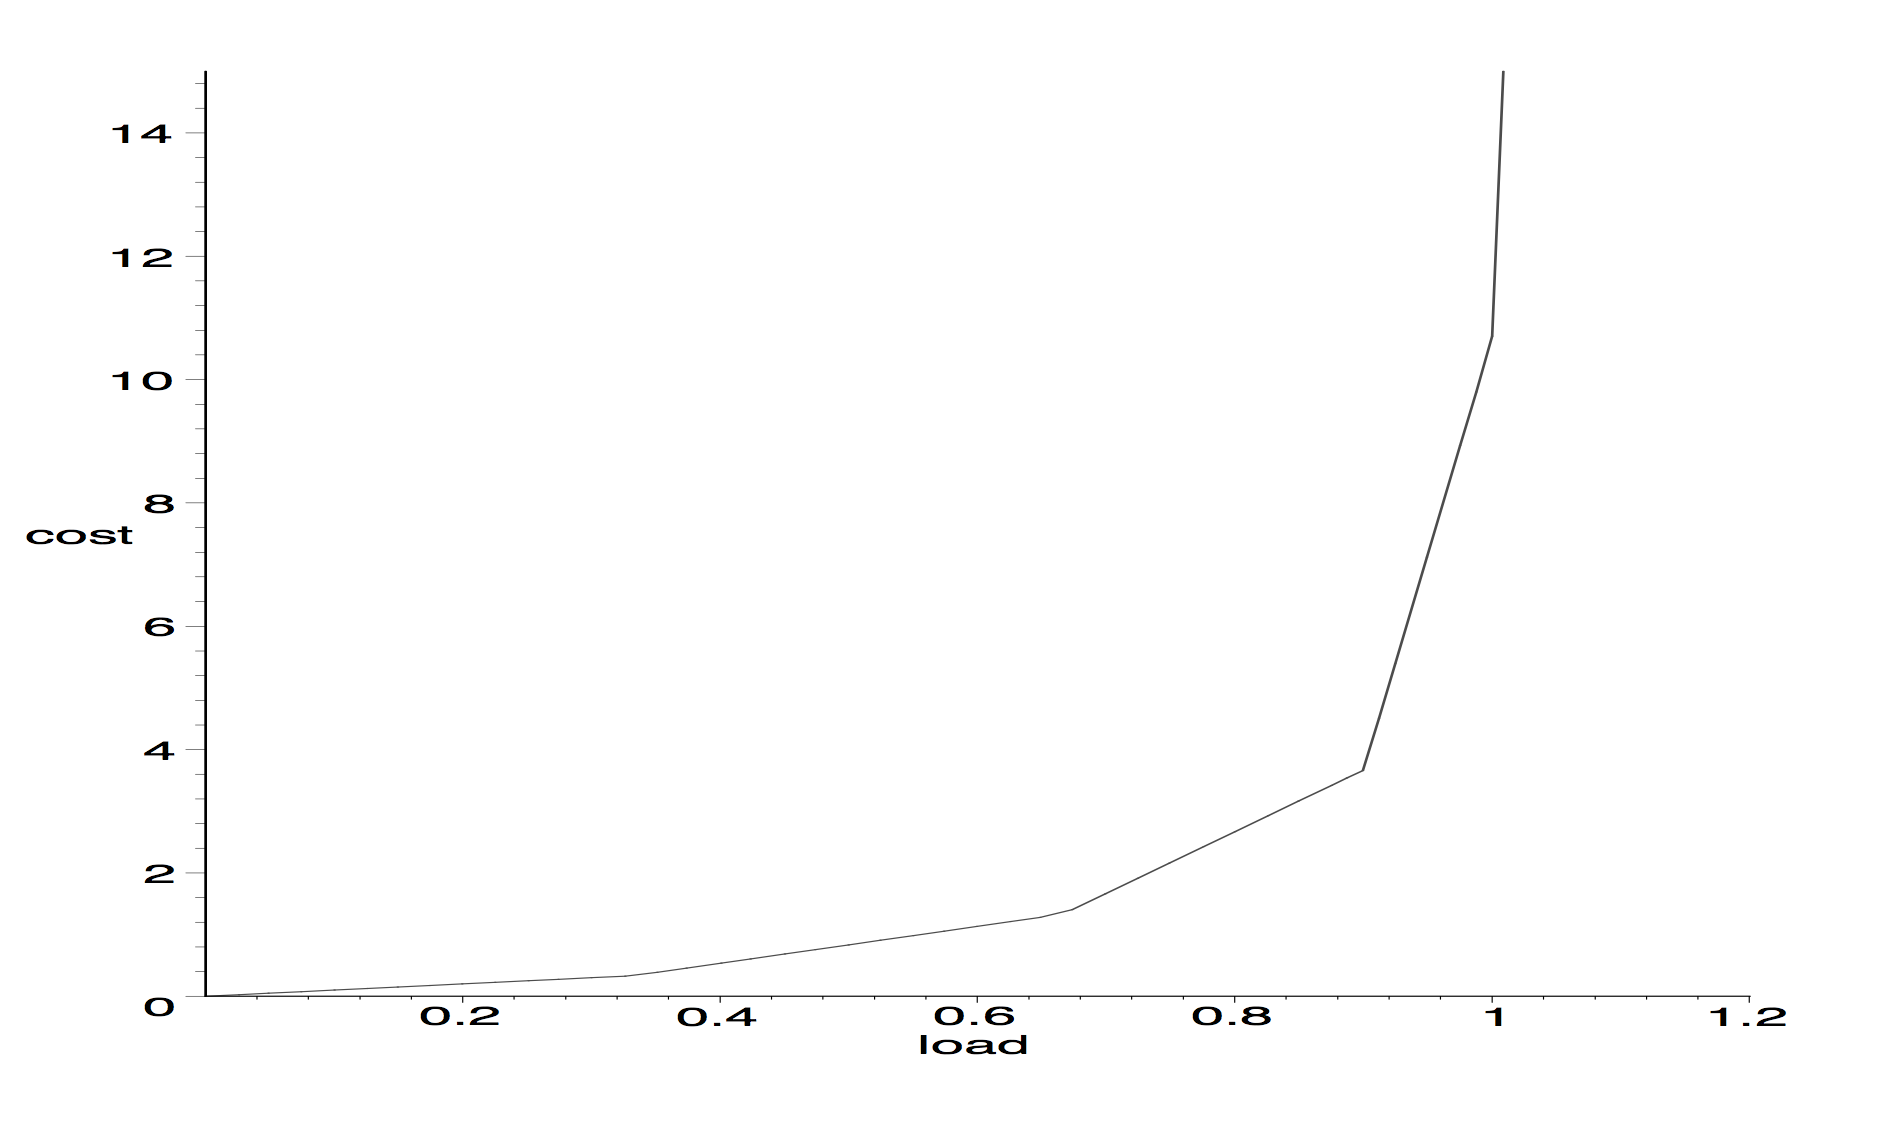
\includegraphics[scale=0.25]{piecewise.png} 
\caption{Cost function for load \label{figure1}}
 \end{figure}
 
 We can apply the same piecewise linear function for node utilization, and the objective function could be minimize 
 $\Phi_e + \Phi_v$.



\section{Design}
\subsection{Optimization Formulation}
To help us understand the problem, we need to simplify the model, instead of focus on minimizing utilization for multi-commodity flows, we only focus on one flow with single source and single destination, and ask the basic question: what a feasible flow really means given a certain network setting. In a graph with of topology (V,E) with both link bandwidth $B(e)$ where $e \in E(u,v)$ and node capacity $C(v)$ where $v \in V$, the workload processed at each node has to be under node constraints while the flow are constrained by link capacity for all links, so 
$\forall v; 0\leq p_v\leq C(v) $ and $\forall e; 0\leq f(e)\leq B(e)$ must be satisfied. In addition to that, we notice that workload is strictly decreasing, given $p(v) = \sum\limits_{in } w(e) - \sum\limits_{out} w(e)$ also holds. The in-network process demand should be carried out by flow, so $\forall e; 0\leq w(e) \leq q*f(e)$ exists. So the formulation is the following:

Minimize  $\Phi_e + \Phi_v$

Subject to
\newline
\begin{subequations}
\begin{align}
&\forall v \in V-\{s, t\}, \sum\limits_i \sum\limits_{in}  f_i(e)= \sum\limits_i  \sum\limits_{out} f_i(e);\\
&\forall e, i, f_i(e) \geq 0;\\
&\forall e, u(e) = \frac{\sum\limits_{i} f_{i}(e) } {B(e)};\\
&\forall e, i, w_i(e) \geq 0,\\
&\forall e, i, w_i(e) \leq q_i* f(e),\\
&\forall v, i, p_i(v) =  \sum\limits_{in } w_i(e) -  \sum\limits_{out} w_i(e) ;\\
&\forall v, i, p_i(v) \geq 0; \\
&\forall v, u(v) = \frac{\sum\limits_{i} p_i(v) } {C(v)} ; \\
&\forall i, \sum\limits_v f_i(s, v) = r_i; \\
&\forall e\in(s, v), i, w_i(e) =q_i* f_i(e);\\
&\forall e\in(v,t), i, w_i(e) =0.
\end{align}
\end{subequations}


Understanding the LP: here (1k, 1j) enforce all flow coming out from source is unprocessed and going to destination are processed. Flow conservation and in-network process handled at each hop are captured in (1a, 1f). We have formally proved the formulation is correct and we can peel the LP solution to path based solution with certain amount of in-network process allocated at each hop.

\subsection{Extended Formulations}
On top of the core formulation we show that some in-network process characteristics can be essentially captured via adding some extra constraints. To keep the math succinct we again only focus on single flow and we assume q=1, and it is intuitive to extend to i flows and any real number q. 

\subsubsection{Flow Size Change after Processing}
The model above shows the model where workload processing does not affect the traffic size. However this is not always the case in networking setting, for example, encryption increase the flow size by a little bit via changing either the header or both header and payload\cite{SIMPLE2013}; compression and transcoding decrease the traffic size by up to a factor of two\cite{Mogul1997}. We need to also put this into our optimization formulation.

There have been some work done regarding flow size change in max flow problems, so called generalized circulation max flow problem.\cite{Wayne1999} Flow circulation model computes the maximum flow coming out source given a network wherein there is an upper bound and lower bound for each link and after each hop the flow size is changed by some factor.  One thing different in our model is that flow size change does not apply for post-processed flows. So here we need to make some change from the previous LP to make the expression more succinct. We divide the flow into two categories; pre-processed, and post-processed. They are represented in $f_1$ and $f_2$ respectively. If we put them back to the $f, w$ presentation, $f_1=w$ and $f_2= f-w$ in model above. Proof for this formulation is similar to core LP.

\textbf{Notations:}

\begin{tabular} {|l |}
\hline
$ f_1(e)=w(e): $ preprocessed flow \\ \hline
$ f_2(e) = f(e)-w(e):$ post-processed flow\\\hline
$t:$ flow size change factor \\ \hline
\end{tabular}
\newline

If there is a size change, at each node, we have $\sum\limits_{in} f_1(e) - \sum\limits_{out}  f_1(e) = p(v)$ and $\sum\limits_{out} f_2(e)-\sum\limits_{in}  f_2(e) = p(v)*t;\;t>0$. Here pre-processed flow equals the amount of workload needing to handle, and post-processed flow equals to pre-processed flow times a factor $r$. Here we can assume factor $r$ is constant for a certain processing and a certain flow. 


\subsubsection{Enforce Policy among Different Middleboxes}
In a network, a flow sometimes needs to go through several different in-network processes, saying firewall->IDS->Proxy, before reaching destination. So far we assume the nodes are all homogeneous, which means they can fulfill all types of tasks or processing. However here we show that this formulation can generalize the problem, including heterogenous hardware middleboxes can also be captured here. If we have specialized hardware for different middleboxes, we will have a new model which contains $C_k(v)$ whereas k represents a type of middlebox processing. 

If we translate network policy into graph, it is essentially serial processing. To ensure serial processing, if we can have several different types of workloads, $w_a$, $w_b\dots$, aside from the workload constraints enforced at section2.1, additional constraints w.r.t. order is needed. To make example simple, assume we only have two different types of in-network process, and we want flow go through process a before process b, then we can simply have $w_a(e) \leq w_b(e)$, in other words, workload demand for a has to be smaller or equal to workload demand for b. 

A simple proof for this formulation is the foliowing:

\textbf{Notations:}

\begin{tabular} {|l |}
\hline
$ f_1=min (w_a, w_b)$\\ \hline
$ f_2 = w_a - w_b$ \\\hline
$ f_3 =w_b - w_a $ \\ \hline
$ f_4 = min (f -w_a ,f - w_b) $ \\ \hline
\end{tabular}
\newline


\begin{proof} Separation of flow can help us better understand the LP. Like $f_1, f_2$ in previous section, here we can have combinatorial of 4 different types of flows. Let us denote $f_1, f_2, f_3, f_4$: pre-A pre-B, pre-A post-B, pre-B post-A, and post-A post-B processed. Since we have  $w_a(e) \leq w_b(e)$ so $f_2\leq 0$, in other words we cannot have any positive flow being processed by b before by a.
\end{proof}
 
 Via the same concept, we can enforce a chain of middleboxes in the Linear Programming formulation. Proof for any number of distinct processes in this formulation can be obtained via induction.


\subsubsection{Middlebox Placement for A Given Network} 
All previous LP formulations assume that link capacity and node capacity B(e) and C(v) are all fixed, but in fact those could be variables; the objective can be to minimize the utilization for each link and node with a sum of B(e) and sum of C(v) equal to some constants. This essentially gives us design choice of where to place middleboxes if we let C(v) be variable. The node processing capacity constraints become $\forall v; 0 \leq C(v) \leq max(v) $ and $\sum\limits_v C(v) = total\;resource$. Again the goal is to minimize $\Phi_e + \Phi_v$. The input becomes flow demands for all flows and the total resource of middlebox pool, and the output becomes resource allocation of middlebox for each node and the routing choice for all flows. Two thing worth noting here is that maybe we need integer/fractional answer for middlebox allocation/flow routing, and putting C(v) at the denominator also loses the linear programming property. However here we emphasize that the problem can be captured in formulation, not integer programming vs. linear programming, we can relax the problem in the following way:
\begin{itemize}
\item To keep the LP property, we can set a hard bound for $\Phi_v$, or in other word, the utilization of each node is bounded by a tunable parameter $\beta$, and here the utility function for middlebox part become minimize the total sum of middlebox, or put in math format: change constraint to $\sum\limits_i p_i(v) \leq \beta*C(v)$ and objective to minimize $\sum\limits_v C(v)$.

\item To solve integer problem from fractional solution, we can round up $C(v)$, if we really want to enforce integer solution for C(v) it would be NP-hard, and there are many well studied techniques for integer approximation solution.
\end{itemize}

\section{Evaluation}


\section{Conclusions}

%\end{document}  % This is where a 'short' article might terminate

%ACKNOWLEDGMENTS are optional
%\section{Acknowledgments}














\bibliographystyle{acm}
\bibliography{references} 

\appendix
\section{Proof for section2.1 LP}
Unlike a simple max flow model this is not very intuitive that our LP formulation is feasible to realize it in path based solution; e.g. it is not easy to find a path to guarantee both link capacity and processing capacity. To achieve it, we need to show two directions:
\begin{itemize}
  \item {\textit{Direction A:} If there is a path-based LP solution, we have an edge-based requirement fulfilled.}
  \item {\textit{Direction B:} If there is an edge-based LP solution, we have a path-based solution.}
\end{itemize}
For \textbf{\textit{Direction A}}, it is easy to show. Once we get a path based solution, we sum up the path-based solution and put it together to a edge-based solution. Through the proof we are using f/w representation for edge-based formulation.

\begin{proof}

For each edge e, $f(e) =\sum\limits_{\pi\in P: e\in \pi} f(\pi)$.

For each node v and each $\pi$, $w(e) = \sum\limits_{e'\in \pi, e' <- e} w(\pi, e')$ (<- means e' is topologically at or after e on the path).

For flow conservation, $ \sum\limits_{(u,v)\in E} f(e) $=$ \sum\limits_{\pi\in P, v\in \pi} f(\pi)$ = $\sum\limits_{(v,w )\in E} f(e)$.

For workload we have:
$w(e) =$ 
$ \sum\limits_{\pi\in P: e'\in \pi, e' \leq e} w(\pi, e')\leq \sum\limits_{\pi\in P: e\in \pi} f(\pi) = f(e).  $\newline
\end{proof}


Next we focus on proof for \textbf{\textit{Direction B}}.

That is, if we have a solution which tells us that if we can assign certain amount of flow and processing 
demand at each edge, we are able to construct paths with a certain amount of flow 
and corresponding processing demand and process workload at every/some node along the path in a certain way.


Setup:
A set of nodes  v$\in$ V, a set of edges e(u,v)$\in$ E. We have the solution of from edge-based LP, with 
f(e) is the flow for each edge and w(e) is workload demand at that edge. We also have processing work at each node p(v) and it is simply $p(v) = 
\sum\limits_{e \in E_{u, v} }w_(e) - \sum\limits_{e \in E_{v, w} }w_(e)  $.

We first build a graph with all vertices \textit{V}, and for $\forall e(u,v) \in E $, if f(e)$ >$0, we put a direct edge e(u,v) in the graph. We might have cycles or even two flows with opposite directions at the same edge. Then we run algorithm [Path Construction] to get one path to allocate flow. For each flow path, we run flow allocation and update the graph, we exhaustively do it until we place all flow and workload demand, this step is essentially captured in algorithm [Flow Placement]. 

We need to prove from two sides for this algorithm: 
\begin{itemize}
  \item {Side 1: there is some node v where p(v) >0, we can always find a path with non-zero flow}
   \item {Side 2: after allocation for one path, constraints are held for the reduced graph} 
\newline
\end{itemize}

To help understand the relation between $p(\pi, e)$ and $f(\pi)$, again we introduce two intermediate variables, $f_1(\pi, e), f_2(\pi, e) $ represents respectively pre processed and post processed flow at edge e on the path $\pi$, so $f_2(\pi, e) =\sum\limits_{e'\; before\;e}p(\pi, e') $ and $ f_1(\pi, e)=f(\pi)- f_2(\pi, e)$, it is not hard to see that $f_2$ is topologically increasing while $f_1$ is topologically decreasing.

Lemma1: If there is a cycle in the path composition, we can achieve in the cycle there are two different edges where one has $min(f_2) = 0$ and one has $min(f_1)=0$. 

\begin{proof} it is similar to flow cancellation in a simpler graph model without workload: 

1. for e=(u,v) whereas $min(f_1) >0$, we can simply cancel the unprocessed flow demand by small amount $\epsilon$, and it does not affect the outcome of the flow outside the loop, while we can reduce the flow load and workload demand in the loop without side effect. 

2. for e=(u,v) whereas $min(f_2)>0$, we can cancel the processed flow demand by small amount $\epsilon$, and this does not affect the outcome of the flow outside of the loop while we can reduce the flow load in the loop without side effect. 


The intuition behind this is that loop exists due to that some flow needs to borrow some processing capacity from some node(s), so it would "detour" a flow with fully unprocessed workload and get back the flow with fully processed workload. 
\end{proof}

Here we introduce an variable $\rho$ for each edge e where $\rho_{e} = \frac{ w(e)}{f(e)}$.

Lemma2
If there is a cycle, we always have one incoming edge with $\rho =1$ and outgoing edge with $\rho =0$ at cross point.

\begin{proof}
If we think this in a $f_1/f_2$ way, $\rho = \frac{ f_1} {f_1+f_2 }$. Here since $f_2=0$ for incoming edge based on lemma1, we have $\rho=1$. The same way to get $\rho_{out}=0$ since $f_1=0$ for outgoing edge. 
\end{proof}

Theorem1: our path composition can always generate path with non-zero flow from source to sink. 

\begin{proof}
\textit{First}, based on lemma1, at some certain node v whereas p(v) >0, there must be some incoming edge with $f_1>0$, the same reason for outgoing edge with $f_2>0$. From source if we keep picking $max(\rho)$ it is a DAG since it cannot get stuck in any loop, so is the same reason for downstream nodes, so it is a combination of two DAGs and thus we can always reach destination from source. 
 
\textit{Second} we need to show for a certain path $\exists e; w(\pi, e)>0$. Since $\delta = min( p(v),$ $w(e_{i}),f(\pi) -w(\pi,e_{i+1}))$; at node v where $p(v)>0$; we have $w(e_i)>0$ because $[\rho_{in} =\frac{ w(e_{in})}{f(e_{in})} ]>\rho_{out}\geq 0$. If $\delta=0$ we have $ f(\pi) -w(\pi,e_{i+1}) =0$, which lead to $ w(\pi, e_{i+1})>0$, otherwise $ \delta>0;w(\pi, e_i) = [ \delta+w(\pi, e_{i+1} )]>0$.

\textit{Finally} our algorithm by design conserve the flow and ensures workload demand is decreasing since w is using backward greedy algorithm.
\end{proof}

This essentially proves \textbf{Side 1}.

Theorem2: flow placement algorithm conserves all the constraints for the reduced graph.

\begin{proof} for LP in section2.1 \newline

(1a)
$\forall v \in \pi; \sum\limits_{in}  f(e) - \sum\limits_{out} f(e)$=
$\sum\limits_{in \not=e_i}  f(e) - \sum\limits_{out\not=e_{i+1} } f(e) +[f(e_i)-f(\pi) ] - [f(e_{i+1}) -f(\pi)] = 0 $

(1b)
$ \forall e \in \pi; f(e) = f(e)-f(\pi) \geq f(e)-f(e) \geq 0$

(1c)
$\forall e \in \pi; f(e) = f(e)-f(\pi) \leq B(e)-f(\pi)=B^{new}(e)$

(1d)
$\forall e \in \pi; w(e) = w(e) - w(\pi, e) \geq w(e) -w(e) \geq 0$

(1e)
$\forall e \in\pi; f(\pi, e)-w(\pi, e) \leq f(e) -w(e) =>w(e) -w(\pi, e) \leq f(e) -f(\pi, e) $

(1g)
$\forall v \in \pi; p(v) = p(v) -\delta \geq p(v) -p(v) \geq 0 $

(1h)
$\forall v \in \pi; p(v) - \delta \leq C(v) - \delta $

$w(\pi, e_1) = f(\pi) $ and $w(\pi, e_k)=0$ are ensured by greedy algorithm, 
\end{proof}
This essentially proves \textbf{Side 2}.


\begin{algorithm}\label {Flow Placement}
\SetAlgoLined
 \KwData{\textit{V, E}, w(e), f(e) for $\forall e \in E$ and p(v) for $\forall v \in V$ }
 \KwResult{f($\pi$), w($\pi$,e) (in which e$\in\pi$) }
\BlankLine
\While{there is one v such that p(v) >0}
{

pick a path $\pi = <e_1, \dots, e_k> $ from Algorithm 2\;
 	$f(\pi) = min( f((e_i) ), \text{ } i\in <1,\dots,k>$\;
	\BlankLine
	w($\pi$)=0\;
	w($\pi, e_k$)=0\;
	\BlankLine
 	\For{$i \leftarrow (k-1)$ \KwTo $1$}
	{
	(u,v)=$e_i$\;
	\emph{//$\delta_i$: workload processed at node i}\;
	$\delta_i = min( p(v), w(e_{i}) , f(\pi) -w(\pi))$\;
	\emph{//Update workload}\;
	$w(\pi, e_i) =\delta_i$\;
	$ w(\pi)= w(\pi)+ \delta_i$\;
	$w(e_i) = w(e_i)- w(\pi)$\;
	$p(v) = p(v)-\delta_i$\;
	$C(v) = C(v) - \delta_i$;
	}
	\BlankLine
	$f(\pi) = w(\pi) $
	\BlankLine
	\emph{//Update flow}\;
	\For{$i \leftarrow (1)$ \KwTo $k$}{
	$f(e_i)=f(e_i)-f(\pi)$\;
	$B(e_i)=B(e_i)-f(\pi)$\;
	}
	
}
\caption{Flow Placement}
\end{algorithm}

\begin{algorithm}\label {Path Construction}
\SetAlgoLined
 \KwData{\textit{V, E}, w(e), f(e) for $\forall e \in E$ and p(v) for $\forall v \in V$ }
 \KwResult{path $\pi$ }
\BlankLine
pick a node v with $p(v)>0$\;
\emph{//Construct path from src->v and v->dest}\;
From v run backward traversal, pick an incoming directed edge with $ max( \rho_{in} )  $ where $\rho_{in} \equiv \frac{ w(e_{in})}{f(e_{in})}$\;
From v run forward traversal, pick an outgoing directed edge with $ min(\rho_{out} ) $ where $\rho_{out} \equiv \frac{ w(e_{out})}{f(e_{out})} $\;
\emph{//See theorem for the reason}\;
\caption{ Path Construction}
\end{algorithm}







\end{document}
